\chapter{Single variable derivatives}

The goal in this chapter is to formalize derivatives of functions whose input is a single real number and whose output is also a single real number. 

\section{Slope of tangent lines}

Let $S$ be a subset of $\R$ and $a \in S$ an interior point. We would like to define the tangent line to the graph of a function $f : S \to \R$ at $a$. We know intuitively what ``tangent line'' should mean: a line that ``just barely touches'' the graph of $f$ at the point $(a, f(a))$. But it's not immediately clear how to formalize this intuition.  

One approach to formalization is to notice that our intuitive idea of ``tangent line'' can be approximated by secant lines, and secant lines can be formalized without ambiguity. More precisely, for small values of $h$, the point $a+h$ is close to $a$ and still in $S$ since $a$ is an interior point of $S$. The slope of the secant line passing through the two points $(a, f(a))$ and $(a+h, f(a+h))$ is computed by the quantity
\[ \frac{f(a+h)-f(a)}{h}. \]
This quantity is often called a \emph{difference quotient}. See \cref{figure-difference-quotient} for a geometric explanation of this difference quotient. By letting $h \to 0$, we get closer and closer to what we intuitively understand to be the slope of the tangent line. 

\begin{figure}
	\begin{center}
	\begin{tikzpicture}
	\begin{axis}[
	xmin=-0.5,xmax=3,
	ymin=-0.5,ymax=2.25,
	ytick={0.7, 1.5},
	xtick={1,2},
	xticklabels={$a$, $a+h$},
	yticklabels={$f(a)$,$f(a+h)$},
	axis lines=middle,
	axis line style=lightgray,
	width=0.75\textwidth
	]
	\addplot[black,style=thick,<->] expression[domain=-0.5:2.45,samples=50]{(x*(x^2+1)+5)/10}; 
	
	
	\addplot[red,<->] expression[domain=0.5:2.4,samples=2]{0.8*(x-1)+0.7}; 
	
	
	\addplot[lightgray,dotted] expression[domain=0:2.75,samples=2]{0.7};
	\addplot[lightgray,dotted] expression[domain=0:2.75,samples=2]{1.5}; 
	\addplot +[mark=none,lightgray,dotted] coordinates {(1, 0) (1, 2)};
	\addplot +[mark=none,lightgray,dotted] coordinates {(2, 0) (2, 2)};
	
	\addplot[gray,dashed] expression[domain=1:2,samples=2]{0.7}; 
	\addplot +[mark=none,gray,dashed] coordinates {(2, 0.7) (2, 1.5)};
	
	\node[color=black,draw=black,circle,fill,inner sep=2pt] at (axis cs:1,0.7) {}; 
	
	\node[color=black,draw=black,circle,fill,inner sep=2pt] at (axis cs:2,1.5) {}; 
	\end{axis}
	\end{tikzpicture}
\end{center}
\caption{The graph of a function $f$ is depicted in black. The secant line passing through the two points $(a, f(a))$ and $(a+h, f(a+h))$ is depicted in red. The ``run'' between these points, is $h$. The ``rise'' between these points is $f(a+h)-f(a)$. Thus the slope of the secant line, computed as ``rise over run,'' is precisely the difference quotient $(f(a+h)-f(a))/h$.}  \label{figure-difference-quotient}
\end{figure}

\begin{definition} \label{single-var-derivative-definition}
	A function $f : S \to \R$ is \emph{differentiable} at an interior point $a \in S$ if 
	\[ \lim_{h \to 0} \frac{f(a+h) - f(a)}{h} \]
	exists. If this limit does exist, its value is called the \emph{derivative of $f$ at $a$}, and is denoted $f'(a)$. 
\end{definition}

\begin{exercise}
	Use the definition of the derivative to determine whether or not each of the following functions $f$ is differentiable at the given point $a$. If it is differentiable, calculate $f'(a)$. Check your answers by making sure they agree with geometric intuition and/or rules you learned during your introductory calculus course. 
	\begin{enumerate}[(a)]
		\item $f(x) = |x|$ at $a = 0$.
		\item $f(x) = x$ at $a = 0$. 
		\item $f(x) = x^2$ at $a = 0$. 
		\item $f(x) = x^2$ at $a = 2$. 
		\item $f(x) = \begin{cases} 1 & x \geq 0 \\ 0 & x < 0 \end{cases}$ at $a = 0$. 
	\end{enumerate}
\end{exercise}

\begin{exercise}[Power rule for positive integer exponents] \label{power-rule-positive}
	Prove that, if $f(x) = x^n$ for a positive integer $n$, then $f'(a) = na^{n-1}$. \textit{Hint.} Recall the binomial theorem, which says that
	\[ (a+h)^n = \sum_{k = 0}^n {n \choose k} a^k h^{n-k}. \]
\end{exercise}

\begin{exercise}[Differentiability implies continuity] \label{differentiable-implies-continuous}
	Prove that if $f : U \to \R$ is differentiable at $a \in U$, then $f$ is also continuous at $a$. 
\end{exercise}

\section{Best linear approximation}

Before proceeding further, we reinterpret the definition of the derivative in a way that will be better suited to generalization to the multivariable setting. Suppose a function $f : S \to \R$ is differentiable at an interior point $a \in S$. The tangent line to the graph at the point $(a, f(a))$ is the graph of the function
\[ t(x) = f'(a)(x-a) + f(a). \]
Since this function $t$ is ``close'' to $f$ near $a$, we should have that
\[ f(a+h)-f(a) \approx t(a+h) - t(a) = f'(a)h \]
for small values of $h$. See \cref{figure-linear-approximation}. 

\begin{figure}
	\begin{center}
		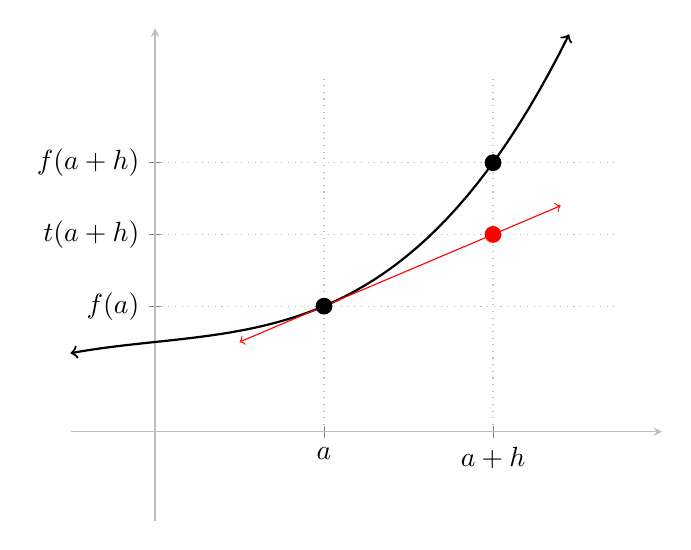
\begin{tikzpicture}
		\begin{axis}[
		xmin=-0.5,xmax=3,
		ymin=-0.5,ymax=2.25,
		ytick={0.7, 1.1, 1.5},
		xtick={1,2},
		xticklabels={$a$, $a+h$},
		yticklabels={$f(a)$, $t(a+h)$, $f(a+h)$},
		axis lines=middle,
		axis line style=lightgray,
		width=0.75\textwidth
		]
		\addplot[black,style=thick,<->] expression[domain=-0.5:2.45,samples=50]{(x*(x^2+1)+5)/10}; 
		
		
		\addplot[red,<->] expression[domain=0.5:2.4,samples=2]{0.4*x+0.3}; 
		
		
		\addplot[lightgray,dotted] expression[domain=0:2.75,samples=2]{0.7};
		\addplot[lightgray,dotted] expression[domain=0:2.75,samples=2]{1.1};
		\addplot[lightgray,dotted] expression[domain=0:2.75,samples=2]{1.5}; 
		\addplot +[mark=none,lightgray,dotted] coordinates {(1, 0) (1, 2)};
		\addplot +[mark=none,lightgray,dotted] coordinates {(2, 0) (2, 2)};
		
		\node[color=black,draw=black,circle,fill,inner sep=2pt] at (axis cs:1,0.7) {}; 
		\node[color=black,draw=black,circle,fill,inner sep=2pt] at (axis cs:2,1.5) {}; 
		\node[color=red,draw=red,circle,fill,inner sep=2pt] at (axis cs:2,1.1) {}; 
		\end{axis}
		\end{tikzpicture}
	\end{center}
	\caption{The graph of a function $f$ is depicted in black, and its tangent line $t$ at $a$ is depicted in red. Then the vertical distance $f(a+h)-f(a)$ is approximated by the vertical distance $t(a+h)-t(a)$. Since the tangent line has slope $f'(a)$, this ``rise'' can be computed as $f'(a)$ times the ``run'' (in other words, $f'(a)h$). As $h$ gets smaller, this approximation gets better.}  \label{figure-linear-approximation}
\end{figure}


Notice that the function $h \mapsto f'(a)h$ is a linear map $\R \to \R$ in the sense of linear algebra. One way to interpret the following result is that the function $h \mapsto f'(a)h$ is the \emph{only} linear map that is a good approximation to $h \mapsto f(a+h)-f(a)$.  

\begin{proposition} \label{unique-linear-single-var}
	A function $f : S \to \R$ is differentiable at an interior point $a \in S$ if and only if there exists a linear map $\ell : \R \to \R$ such that
	\[ |f(a+h)-f(a) - \ell(h)| = o(|h|) \text{ as } h \to 0. \]
	Moreover, if there exists such a linear map $\ell$, then $\ell$ is uniquely determined: it must be given by \[ \ell(h) = f'(a)h \]
	for all $h \in \R$. 
\end{proposition}

\begin{proof}
	Let $\ell$ be a linear map $\ell(h) = ch$, where $c$ is some scalar. Observe that
	\[ \begin{aligned} \frac{|f(a+h)-f(a)-\ell(h)|}{|h|} &= \left| \frac{f(a+h)-f(a) - ch}{h} \right| \\
	&= \left| \frac{f(a+h)-f(a)}{h} - c \right|. \end{aligned} \]
	This leads to the following sequence of ``if and only if'' statements. 
	\[ \begin{aligned} |f(a+h)-f(a)-\ell(h)| = o(|h|) &\iff \lim_{h \to 0} \frac{|f(a+h)-f(a)-\ell(h)|}{|h|} = 0 \\
	&\iff \lim_{h \to 0} \left| \frac{f(a+h)-f(a)}{h} - c \right| = 0 \\
	&\iff \lim_{h \to 0} \left( \frac{f(a+h)-f(a)}{h} - c \right) = 0 \\
	&\iff \lim_{h \to 0} \frac{f(a+h)-f(a)}{h} = c \end{aligned} \]
	The statement of the proposition follows. 
\end{proof}

\begin{definition}
	If $f : S \to \R$ is differentiable at an interior point $a \in U$, we define $df_a : \R \to \R$ to be the linear map $df_a(h) = f'(a)h$. 
\end{definition}

In other words, $df_a$ is the only good linear approximation to the function $h \mapsto f(a+h)-f(a)$. Being the only good linear approximation, it is also the best linear approximation, whence the name of this section. 

\section{Rules of differentiation}


The goal in this section is to prove the rules for differentiation that one encounters in an introductory calculus course. 

\subsection{Sum and scalar multiples rule}

Both of the following can be proved using either the definition of the derivative \ref{single-var-derivative-definition} or the equivalent ``best linear approximation'' characterization of \cref{unique-linear-single-var}. My suggestion is that you try both methods for both of these exercises. When you use \cref{unique-linear-single-var}, you may find \cref{little-o-vector-space} useful. 

\begin{exercise}[Sum rule] \label{sum-rule}
	Prove that, if $f, g : S \to \R$ are both differentiable at an interior point $a \in U$, then $f + g$ is also differentiable at $a$ and \[ (f+g)'(a) = f'(a) + g'(a). \]
\end{exercise}

\begin{exercise}[Scalar multiples rule] \label{scalar-multiples-rule}
	Prove that, if $c$ is a constant and $f : S \to \R$ is differentiable at an interior point $a \in S$, then $cf$ is also differentiable at $a$ and \[ (cf)'(a) = c f'(a). \]
\end{exercise}

\subsection{Product and quotient rules}

\begin{proposition}[Product rule]
	Suppose $f, g : U \to \R$ are both differentiable at $a \in U$. Then $fg$ is also differentiable at $a$ and 
	\[ (fg)'(a) = f'(a)g(a) + f(a)g'(a). \]
\end{proposition}

\begin{proof}
	The proof is a clever algebraic manipulation of difference quotients. The key trick is introducing a ``cross term'' of the form $f(a)g(a+h)$, and then cancelling it out by also introducing its negative. More precisely, for any sufficiently small real number $h$, we have 
	\[ \begin{aligned} \frac{(fg)(a+h)-(fg)(a)}{h} &= \frac{f(a+h)g(a+h) - f(a)g(a)}{h} \\ 
	&= \frac{f(a+h)g(a+h) {\color{blue}-f(a)g(a+h) + f(a)g(a+h)} - f(a)g(a)}{h} \\
	&= \frac{f(a+h)g(a+h) - f(a)g(a+h)}{h} + \frac{f(a)g(a+h) - f(a)g(a)}{h} \\
	&= \frac{f(a+h) - f(a)}{h} \cdot g(a+h) + f(a) \cdot \frac{g(a+h) - g(a)}{h}. \end{aligned} \]
	Taking the limit as $h \to 0$ yields the result. 
\end{proof}

\begin{exercise}
	Check your understanding of the above proof of the product rule. 
\begin{enumerate}[(a)]
	\item Could you have instead introduced a cross term of the form $f(a+h)g(a)$?
	\item At what point is \cref{differentiable-implies-continuous} tacitly used in the above proof?
\end{enumerate}
\end{exercise}

\begin{exercise}
	 Reprove the scalar multiples rule (\cref{scalar-multiples-rule}) using the product rule. 
\end{exercise}

\begin{exercise}[Quotient rule] \label{quotient-rule}
	Suppose $f, g : S \to \R$ are both differentiable at an interior point $a \in U$, and that $g(a) \neq 0$. Prove that $f/g$ is also differentiable at $a$ and 
	\[ (f/g)'(a) = \frac{f'(a)g(a) - f(a)g'(a)}{g(a)^2}. \] 
	\textit{Hint.} Observe that \[ \frac{(f/g)(a+h)-(f/g)(a)}{h} = \frac{\frac{f(a+h)}{g(a+h)} - \frac{f(a)}{g(a)} }{h}. \]
	Multiply both the numerator and denominator by $g(a+h)g(a)$ to clear the denominators inside the numerator, and then introduce the cross term $f(a)g(a)$. Be sure to notice at what point you use \cref{differentiable-implies-continuous}.
\end{exercise}

\begin{comment}
	Again, the proof is a clever algebraic manipulation of difference quotients! There are now two tricks: clearing denominators, and then introducing a cross term $f(a)g(a)$. 
	\[ \begin{aligned} \frac{(f/g)(a+h)-(f/g)(a)}{h} &= \frac{\frac{f(a+h)}{g(a+h)} - \frac{f(a)}{g(a)} }{h} \\ 
	&= \frac{g(a+h)g(a)}{g(a+h)g(a)} \cdot \frac{\frac{f(a+h)}{g(a+h)} - \frac{f(a)}{g(a)} }{h} \\
	&= \frac{1}{g(a+h)g(a)} \frac{f(a+h)g(a) - f(a)g(a+h)}{h} \\
	&= \frac{1}{g(a+h)g(a)} \frac{f(a+h)g(a) {\color{blue}- f(a)g(a) + f(a)g(a)} - f(a)g(a+h)}{h} \\ 
	&= \frac{1}{g(a+h)g(a)} \left( \frac{f(a+h)g(a) - f(a)g(a)}{h} + \frac{f(a)g(a) - f(a)g(a+h)}{h} \right) \\
	&= \frac{1}{g(a+h)g(a)} \left( \frac{f(a+h) - f(a)}{h} \cdot g(a) + f(a) \cdot \frac{g(a) - g(a+h)}{h} \right) \end{aligned} \]
\end{comment}

\begin{exercise}[Power rule for integer exponents] \label{power-rule-integer}
	Extend the result of \cref{power-rule-positive} to arbitrary integer exponents. \textit{Hint.} Use the quotient rule for negative integers. The exponent zero is a special case; deal with it separately. 
\end{exercise}

\subsection{Chain rule}

\begin{proposition}[Chain rule] \label{chain-rule-single}
	Suppose that $S$ and $T$ are both subsets of $\R$, that $f : S \to T$ is differentiable at an interior point $a$, that $f(a)$ is an interior point of $T$, and that $g : T \to \R$ is differentiable at $f(a)$. Then the composite $g \circ f : S \to \R$ is also differentiable at $a$, and 
	\[ (g \circ f)'(a) = g'(f(a))f'(a). \]
\end{proposition}

Let us discuss two different proofs of this important result. 

\subsubsection*{First proof}

The first proof uses the definition of the derivative \ref{single-var-derivative-definition}, but there is a subtle technicality involved; so, let us discuss it informally first before diving into the formal proof.  

The idea involved is again a clever rewriting of difference quotients. Again, we introduce a cross term, which in this is $f(a+h) - f(a)$. But this time we introduce this cross term ``multiplicatively'' rather than ``additively.'' More precsiely, we have
\[ \begin{aligned} \frac{(g \circ f)(a+h) - (g \circ f)(a)}{h} &= \frac{g(f(a+h)) - g(f(a))}{h} \\ &= \frac{g(f(a+h)) - g(f(a))}{f(a+h)-f(a)} \cdot \frac{f(a+h)-f(a)}{h}. \end{aligned} \]
The difference quotient on the right is precisely $f'(a)$. Thus, it would be sufficient to prove  
\begin{equation} \label{wrong-conjecture} \lim_{h \to 0} \frac{g(f(a+h)) - g(f(a))}{f(a+h)-f(a)} = g'(f(a)). \end{equation}
This formula looks an awful lot like the difference quotient that is used to define the derivative of $g$ at $f(a)$. In fact, since $f$ is continuous at $a$ by \cref{differentiable-implies-continuous}, we have $f(a+h) \approx f(a)+h$ for small values of $h$, which means that
\[ \frac{g(f(a+h)) - g(f(a))}{f(a+h)-f(a)} \approx \frac{g(f(a)+h) - g(f(a))}{f(a)+h-f(a)} = \frac{(g \circ f)(a+h) - (g\circ f)(a)}{h} \]
for small values of $h$. Taking the limit as $h \to 0$ on the right-hand side yields precisely $g'(f(a))$, so \cref{wrong-conjecture} seems like a reasonable conjecture. 

The problem is that \cref{wrong-conjecture} isn't true. Issues arise when $f(a+h) = f(a)$ for arbitrarily small values of $h$, which leads to an infinite sequence of divisions by 0. 

\begin{example}
	Let \[ f(x) = \begin{cases} x^2\sin(1/x) & \text{if } x \neq 0 \\ 0 & \text{if } x = 0 \end{cases} \] and let $g(x) = x^2$. Observe that $g'(f(0)) = 0$. You will show later (in \cref{power-times-sine}) that $f$ is in fact differentiable at 0, so these functions do satisfy the hypothesis of the chain rule. However, the limit as $h \to 0$ of
	\[ \frac{g(f(a+h)) - g(f(a))}{f(a+h)-f(a)} = \frac{(h^2\sin(1/h))^2}{h^2\sin(1/h)} \]
	does not exist. For example, the sequence $h_k = 1/k\pi$ converges to 0 as $k \to \infty$, but the expression above is undefined along this sequence. 
\end{example}

We will get around the kind of issue that is described by the above example by carefully studying the expression
\begin{equation} \label{weird-difference-quotient} \frac{g(f(a+h)) - g(f(a))}{f(a+h)-f(a)}. \end{equation}
Observe that, when $f(a+h)\neq f(a)$, then this expression is precisely the difference quotient that calculates the slope of the secant line passing through $(f(a), g(f(a))$ and $(f(a+h), g(f(a+h))$. When $f(a+h) = f(a)$, this secant line doesn't make sense; but what does make sense is the tangent line! So we'll remove the undefinedness of expression \eqref{weird-difference-quotient} by extending it so that it takes the value $g'(f(a))$ whenever $f(a+h) = f(a)$. 

This leads us to our first proof of the chain rule. 

\begin{proof}[First proof of the chain rule]
	Consider the function $\epsilon$ defined for small values of $h$ by $\epsilon(h) = f(a+h)-f(a)$. See \cref{value-difference-chain-rule}. You will verify in \cref{chain-rule-details} below that $\epsilon$ is continuous at 0. 
	
	
	\begin{figure}
		\begin{center}
			\begin{tikzpicture}
			\begin{axis}[
			xmin=-0.5,xmax=3,
			ymin=-0.5,ymax=2.25,
			ytick={0.7, 1.5},
			xtick={1,2},
			xticklabels={$a$, $a+h$},
			yticklabels={$f(a)$,$f(a+h)$},
			axis lines=middle,
			axis line style=lightgray,
			width=0.75\textwidth
			]
			\addplot[black,style=thick,<->] expression[domain=-0.5:2.45,samples=50]{(x*(x^2+1)+5)/10}; 
			
			
			\addplot[lightgray,dotted] expression[domain=0:2.75,samples=2]{0.7};
			\addplot[lightgray,dotted] expression[domain=0:2.75,samples=2]{1.5}; 
			\addplot +[mark=none,lightgray,dotted] coordinates {(1, 0) (1, 2)};
			\addplot +[mark=none,lightgray,dotted] coordinates {(2, 0) (2, 2)};
			
			
			\node[color=black,draw=black,circle,fill,inner sep=2pt] at (axis cs:1,0.7) {}; 
			
			\node[color=black,draw=black,circle,fill,inner sep=2pt] at (axis cs:2,1.5) {}; 
			
			
			\addplot +[mark=none,gray,red,<->,solid] coordinates {(2, 0.7) (2, 1.5)};
			\end{axis}
			\end{tikzpicture}
		\end{center}
		\caption{The graph of $f$ is depicted in black. The value of the function $t$ on a small nonzero input value $h$ is the vertical distance depicted in red.}  \label{value-difference-chain-rule}
	\end{figure}

	Next, define a function $\sigma$ by the following.  
	\[ \sigma(k) = \begin{cases} \dfrac{g(f(a)+k) - g(f(a))}{k} & \text{if } k \neq 0 \\ g'(f(a)) & \text{if } k = 0 \end{cases} \]
	In other words, $\sigma$ is the function that, on some small nonzero input $k$, outputs the slope of the secant line connecting the two points on the graph of $g$ where $x = f(a)$ and $x = f(a) + k$. See \cref{slope-function-chain-rule}. It follows from the definition of the derivative of $g$ at $f(a)$ that the function $\sigma$ is continuous at 0. 
	
	\begin{figure}
		\begin{center}
			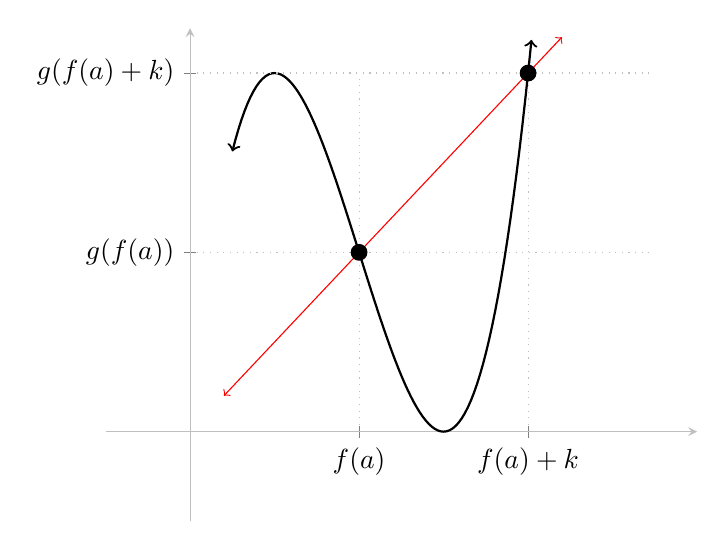
\begin{tikzpicture}
			\begin{axis}[
			xmin=-0.5,xmax=3,
			ymin=-0.5,ymax=2.25,
			ytick={1, 2},
			xtick={1,2},
			xticklabels={$f(a)$, $f(a)+k$},
			yticklabels={$g(f(a))$,$g(f(a)+k)$},
			axis lines=middle,
			axis line style=lightgray,
			width=0.75\textwidth
			]
			\addplot[black,style=thick,<->] expression[domain=0.25:2.02,samples=100]{4*x^3-12*x^2+9*x}; 
			
			
			\addplot[red,<->] expression[domain=0.2:2.2,samples=2]{(x-1)+1}; 
			
			
			\addplot[lightgray,dotted] expression[domain=0:2.75,samples=2]{1};
			\addplot[lightgray,dotted] expression[domain=0:2.75,samples=2]{2}; 
			\addplot +[mark=none,lightgray,dotted] coordinates {(1, 0) (1, 2)};
			\addplot +[mark=none,lightgray,dotted] coordinates {(2, 0) (2, 2)};
			
			\node[color=black,draw=black,circle,fill,inner sep=2pt] at (axis cs:1,1) {}; 
			
			\node[color=black,draw=black,circle,fill,inner sep=2pt] at (axis cs:2,2) {}; 
			\end{axis}
			\end{tikzpicture}
		\end{center}
		\caption{The graph of $g$ is depicted in black. The output of the function $s$ on a small nonzero input value $h$ is the slope of the red secant line passing through the two points $(f(a), g(f(a))$ and $(f(a)+k, g(f(a)+k))$. }  \label{slope-function-chain-rule}
	\end{figure}
	
	
	Observe that
	\begin{equation} \label{alternative-to-multiplicative-cross-term} \frac{(g \circ f)(a+h) - (g \circ f)(a)}{h} = \sigma(\epsilon(h)) \cdot \frac{f(a+h)-f(a)}{h} \end{equation}
	for all small values of $h$, as you will verify in \cref{chain-rule-details} below. Thus
	\[ \begin{aligned} \lim_{h \to 0} \frac{(g \circ f)(a+h) - (g \circ f)(a)}{h} &= \lim_{h \to 0} \sigma (\epsilon(h)) \cdot \frac{f(a+h)-f(a)}{h} \\ 
	&\stackrel{(*)}{=} \sigma (\epsilon(0)) f'(a) \\
	&= g'(f(a)) f'(a) \end{aligned}  \]
	where we have used the continuity of $\epsilon$ and $\sigma$ and the definition of the derivative of $f$ at $a$ for the step labeled $(*)$ above. This proves the chain rule. 
\end{proof}
	
\begin{exercise} \label{chain-rule-details}
	Verify the missing details in the above proof. Specifically, check the following. 
	\begin{enumerate}[(a)]
		\item Prove that $\epsilon$ is continuous at 0.
		\item Prove \cref{alternative-to-multiplicative-cross-term}. \textit{Hint.} As suggested by our analysis before the proof of the chain rule, split up your proof of \cref{alternative-to-multiplicative-cross-term} into two cases: when $f(a+h) \neq f(a)$, and when $f(a+h) = f(a)$. 
	\end{enumerate}
\end{exercise}

\subsubsection*{Second proof}

Our second proof of the chain rule will use the ``best linear approximation'' interpretation of derivatives provided by \cref{unique-linear-single-var}. 

\begin{proof}[Second proof of the chain rule] \renewcommand{\qedsymbol}{}
	By \cref{unique-linear-single-var}, it is sufficient to prove that
	\[ g(f(a+h))-g(f(a))-dg_{f(a)}(df_a(h)) = o(|h|) \text{ as } h \to 0. \]
	Define the following ``error in approximation'' functions. 
	\[ \begin{aligned} 
	r(h) &= f(a+h)-f(a) - df_a(h) \\ 
	s(k) &= g(f(a)+k)-g(f(a))-dg_{f(a)}(k) \end{aligned}\]
	See \cref{figure-error-in-approximation}. 
	
	\begin{figure}
		\begin{center}
			\begin{tikzpicture}
			\begin{axis}[
			xmin=-0.5,xmax=3,
			ymin=-0.5,ymax=2.25,
			ytick={0.7, 1.1, 1.5},
			xtick={1,2},
			xticklabels={$a$, $a+h$},
			yticklabels={$f(a)$, $f(a)+df_a(h)$, $f(a+h)$},
			axis lines=middle,
			axis line style=lightgray,
			width=0.75\textwidth
			]
			\addplot[black,<->] expression[domain=-0.5:2.45,samples=50]{(x*(x^2+1)+5)/10}; 
			
			
			\addplot[black,<->] expression[domain=0.5:2.4,samples=2]{0.4*x+0.3}; 
			
			
			\addplot[lightgray,dotted] expression[domain=0:2.75,samples=2]{0.7};
			\addplot[lightgray,dotted] expression[domain=0:2.75,samples=2]{1.1};
			\addplot[lightgray,dotted] expression[domain=0:2.75,samples=2]{1.5}; 
			\addplot +[mark=none,lightgray,dotted] coordinates {(1, 0) (1, 2)};
			\addplot +[mark=none,lightgray,dotted] coordinates {(2, 0) (2, 2)};
			
			
			\node[color=black,draw=black,circle,fill,inner sep=2pt] at (axis cs:1,0.7) {}; 
			\node[color=black,draw=black,circle,fill,inner sep=2pt] at (axis cs:2,1.5) {}; 
			\node[color=black,draw=black,circle,fill,inner sep=2pt] at (axis cs:2,1.1) {}; 
			
			
			\addplot +[mark=none,red,solid,style=thick,<->] coordinates {(2, 1.1) (2, 1.5)};
			\end{axis}
			\end{tikzpicture}
		\end{center}
		\caption{The graphs of a function $f$ and its tangent line $f(a) + df_a$ are depicted in red. On a small input $h$, the ``error in approximation'' function $r$ outputs the vertical distance indicated in red.}  \label{figure-error-in-approximation}
	\end{figure}

	Since
	\[ f(a+h) = f(a) + df_a(h) + r(h) \]
	by definition of $r$, we have
	\[ \begin{aligned}
	g(f(a+h)) &= g(f(a) + df_a(h) + r(h)) \\
	&= g(f(a)) + dg_{f(a)}(df_{a}(h) + r(h)) + s(df_a(h)+r(h)) \\
	&= g(f(a)) + dg_{f(a)}(df_{a}(h)) + dg_{f(a)}(r(h)) +  s(df_a(h) + r(h)) \end{aligned} \]
	where we use the definition of $s$ on input $k = df_a(h)+r(h)$ for the second step, and the fact that $dg_{f(a)}$ is linear for the third. Thus
	\[ g(f(a+h)) - g(f(a)) - dg_{f(a)}(df_a(h)) = dg_{f(a)}(r(h)) + s(df_a(h)+r(h)). \]
	We therefore want to prove that the right-hand side is $o(|h|)$. 	
	
	Since \[ dg_{f(a)}(r(h)) = g'(f(a)) \cdot r(h) \] is just a scalar multiple of $r$, and $r = o(|h|)$, we see that $dg_{f(a)}(r) = o(|h|)$ also. So it is sufficient to prove that
	\[ s(df_a(h)+r(h)) = o(|h|). \]
	We've now hit the technical part, so let's hit pause. 
\end{proof}

To see why this is technical, and for essentially the same reasons as the previous proof, notice that we're trying to prove that
\[ \lim_{h \to 0} \frac{|s(df_a(h)+r(h)|)}{|h|} = 0.  \]
To prove this, it's tempting to introduce a multiplicative cross-term as follows. 
\[ \frac{|s(df_a(h)+r(h)|)}{|h|} = \frac{|s(df_a(h)+r(h)|)}{|df_a(h)+r(h)|} \cdot \frac{|df_a(h)+r(h)|}{|h|} \]
But notice that $df_a(h)+r(h) = f(a+h)-f(a)$ by definition of $r$, so this cross term is problematic for the same reasons as before! If $f(a+h) = f(a)$ for $h$ arbitrary close to $0$, we have an infinite sequence of divisions by zeroes that causes problems. 

We'll deal with this problem in essentially the same way as before: namely, we extend the definition of 
\[\frac{|s(df_a(h)+r(h)|)}{|df_a(h)+r(h)|}\]
so that it is also defined when $f(a+h) = f(a)$. 

\begin{proof}[Second proof of the chain rule, continued]
	Define $\eta(k) = s(k)/k$. Observe that $\eta(0) = 0$. Moreover, since $s(k) = o(|k|)$ by \cref{unique-linear-single-var}, we see that $\eta$ is continuous at 0. Then 
	\[ \begin{aligned} \frac{|s(df_a(h)+r(h))|}{|h|} &= \frac{|\eta(df_a(h)+r(h))| \cdot |df_a(h)+r(h)|}{|h|} \\
	&\leq |\eta(df_a(h)+r(h))| \cdot \left( |f'(a)| + \frac{|r(h)|}{|h|} \right). \end{aligned} \]
	Observe that $df_a + r$ is continuous at $0$ by \cref{chain-rule-proof-2-details} below; moreover, we have just seen that $\eta$ is continuous at $(df_a + r)(0) = 0$. Thus the composite $\eta \circ (df_a + r)$ is also continuous at 0. Thus
	\[ \lim_{h \to 0} |\eta(df_a(h)+r(h))| \cdot \left( |f'(a)| + \frac{|r(h)|}{|h|} \right) = 0, \]
	where we have used the fact that $|r(h)| = o(|h|)$ to see that the parenthetical expression has a finite limit (namely, $|f'(a)|$). So, by the squeeze theorem, we can therefore conclude that $|s(df_a(h)+r(h))| = o(|h|)$.  
\end{proof}

\begin{comment}[Second proof of the chain rule, continued]
	To prove that \[ s(df_a(h)+r(h)) = o(|h|), \] let's whip out some epsilons and deltas. Suppose $\epsilon > 0$. We want to find a $\delta > 0$ such that $|h| < \delta$ implies that
	\[ |s(df_a(h)+r(h))| \leq \epsilon|h|. \]
	
	Since $s$ is $o(|h|)$, we know that for any $\epsilon_1 > 0$ there exists $\delta_1 > 0$ such that $|k| < \delta_1$ implies that
	\[ \begin{aligned} |s(k)| \leq \epsilon_1|k|. \end{aligned} \] 
	Since $df_a + r$ is continuous at 0, there then exists $\delta_2 > 0$ such that $|h| < \delta$ implies that $|df_a(h) + r(h)| < \delta_1$. Then for $|h| < \delta_2$, we have
	\[ |s(df_a(h) + r(h)| \leq \epsilon_1 |df_a(h) + r(h)| 
	\leq \epsilon_1|f'(a)||h| + \epsilon_1|r(h)| \]
	Since $r$ is $o(|h|)$, for any $\epsilon_2 > 0$ there exists $\delta_3 > 0$ such that $|h| < \delta_3$ implies that $|r(h)| \leq \epsilon_2 |h|$. Let $\delta = \min\{\delta_2, \delta_3\}$. Then for $|h| < \delta$, we can continue the above chain of inequalities to obtain 
	\[ |s(df_a(h) + r(h)| \leq \epsilon_1|f'(a)||h| + \epsilon_1 \epsilon_2|h| = \epsilon_1(|f'(a)| + \epsilon_2)|h|. \]
	So we let $\epsilon_2 = 1$ and then let 
	\[ \epsilon_1 = \frac{\epsilon}{|f'(a)| + 1}. \]
	The $\delta$ obtained by going through the above process then has the desired property. 
\end{comment}

\begin{exercise} \label{chain-rule-proof-2-details}
	Check that the function $r$ is continuous at 0.
\end{exercise}

Notice that in the first proof, the trick to overcoming the technicality was defining the function $\sigma$ at $k = 0$. In the second proof, the trick to overcoming the same technicality was defining $\eta$ at $k = 0$. These tricks are really the same trick, as shown by the following.  

\begin{exercise}
	Prove that the function $\eta$ from the second proof and the function $\sigma$ from the first proof are related by the equation
	\[ \sigma(k) = g'(f(a)) + \eta(k). \]
\end{exercise}

\subsubsection*{Applications of the chain rule}

\begin{exercise}[Derivatives of inverses] \label{inverse-derivative}
	Suppose $S$ and $T$ are both subsets of $\R$ and $f : S \to T$ is bijective, with inverse function $f^{-1} : T \to S$. Suppose further that $f$ is differentiable at an interior point $a \in S$, that $f'(a) \neq 0$, and that $b = f(a)$ is an interior point of $T$. Prove that $f^{-1}$ is differentiable at $b$ and
	\[ (f^{-1})'(b) = \frac{1}{f'(a)}. \]
\end{exercise}

\begin{exercise}[Power rule for fractional exponents] \label{power-rule-fractional}
	Extend the result of \cref{power-rule-integer} to arbitrary rational exponents (ie, to exponents that can be written in the form $m/n$ where $m$ and $n$ are both integers). 
\end{exercise}

\subsection{Some rules without proofs}

Here are some other rules you probably remember from calculus. We won't prove them here, but you should feel free to use them. 
\begin{enumerate}[(1)]
	\item If $f(x) = e^x$, then $f'(x) = e^x$. 
	\item If $f(x) = \ln(x)$, then $f'(x) = 1/x$. 
	\item If $f(x) = \sin(x)$, then $f'(x) = \cos(x)$. 
	\item If $f(x) = \cos(x)$, then $f'(x) = -\sin(x)$. 
	\item If $f(x) = x^r$ for some \emph{real} number $r$, then $f'(x) = rx^{r-1}$. 
\end{enumerate}
Note that by doing \cref{power-rule-fractional}, you have already proved the most common cases of the power rule (5). 

The proofs of these facts are omitted not because the proofs are particularly difficult, but because we would have to go on a long detour to even define the functions involved sufficiently rigorously to prove anything about them. That would distract us from our object of meditation.

\begin{exercise} \label{power-times-sine}
	\begin{enumerate}[(a)]
		\item Prove that the function \[ f_1(x) = \begin{cases} x\sin(1/x) & \text{if } x \neq 0 \\ 0 & \text{if } x = 0 \end{cases} \]
		is continuous at 0 but is not differentiable at 0. In particular words, $f \in C^0(\R) \setminus C^1(\R)$. 
		\item Prove that the function \[ f_2(x) = \begin{cases} x^2\sin(1/x) & \text{if } x \neq 0 \\ 0 & \text{if } x = 0 \end{cases} \]
		is differentiable at 0 but the derivative $f_2'$ is not continuous at 0.  
	\end{enumerate} 
\end{exercise} 

\section{Levels of differentiability} 

\subsection{$C^n$ functions}

\begin{definition}
	Suppose $U$ is an open subset of $\R$ and $f : U \to \R$ is a function. Then $f$ is \emph{differentiable} if $f$ is differentiable at every $a \in U$. If the function $f' : U \to \R$ is also continuous, then $f$ is \emph{continuously differentiable}. 
\end{definition}

\begin{definition}
	Let $U$ be an open subset of $\R$. For any non-negative integer $n$, we define the set $C^n(U)$ inductively as follows. 
	\begin{itemize}
		\item $C^0(U)$ is the set of continuous functions $f : U \to \R$. 
		\item $C^1(U)$ is the set of functions $f$ such that $f'$ exists and is in $C^0(U)$. Concretely, this means that $f$ is continuously differentiable. 
		\item $C^2(U)$ is the set of functions $f : U \to \R$ such that the derivative $f'$ exists and is in $C^1(U)$. Concretely, this means that the the derivative of the derivative $(f')'$, called the \emph{second derivative} of $f$ and written $f''$ or $f^{(2)}$, exists and is continuous on $U$. 
		\item In general, $C^{n+1}(U)$ is the set of functions $f : U \to \R$ such that $f'$ exists and is in $C^n(U)$. This means that the \emph{$(n+1)$st derivative} $f^{(n+1)} = (f^{(n)})'$ exists and is continuous on $U$.
	\end{itemize}
\end{definition}

\begin{exercise}
	Prove that, for every non-negative integer $n$, $C^n(U)$ is a subspace of the vector space of all functions $U \to \R$. 
\end{exercise}

\begin{exercise}
	Prove that, if $f, g \in C^n(U)$, then the product $fg$ is also in $C^n(U)$. 
\end{exercise}

We have an infinite chain of inclusions
\[ \{\text{all functions } U \to \R\} \supseteq C^0(U) \supseteq C^1(U) \supseteq C^2(U) \supseteq C^3(U) \supseteq \dotsb. \]
The following exercise shows that all of these inclusions are strict; in other words $C^n(U) \supseteq C^{n+1}(U)$ for all $n$. 

\begin{exercise}
	For every non-negative integer $n$, let 
	\[ f_n(x) = x^n|x|. \]
	Prove that $f_n$ is in $C^n(\R)$ but not $C^{n+1}(\R)$. \textit{Hint.} Prove that $f_{n+1}' = (n+2)f_n$. Then use induction. 
\end{exercise}

\subsection{Smooth functions}

\begin{definition}
	A function $f : U \to \R$ is \emph{infinitely differentiable} or \emph{smooth} if it is in $C^n(U)$ for all $n$. The set of smooth functions is denoted $C^\infty(U)$ or $\O(U)$. 
\end{definition}

\begin{exercise} \label{canonical-bump}
	Consider the function $\psi : \R \to \R$ defined as follows.  
	\[ \psi(x) = \begin{cases} e^{1/(x^2-1)} & \text{if } -1 < x < 1 \\ 0 & \text{otherwise} \end{cases} \]
	See \cref{canonical-bump-graph} for its graph. Prove that $\psi$ is smooth. \textit{Hint.} First prove directly from definitions that $\psi$ is continuously differentiable. Then use induction to prove that it is in $C^n(\R)$ for all $n$. 
	
	\begin{figure}
		\begin{center}
			\begin{tikzpicture}
			\begin{axis}[
			xmin=-1.5,xmax=1.5,
			ymin=-0.1,ymax=0.5,
			ytick={0},
			xtick={-1,1},
			xticklabels={$-1$,1},
			yticklabels={},
			axis lines=middle,
			axis line style=lightgray,
			width=0.75\textwidth
			]
			
			
			\addplot[black,style=thick] expression[domain=-1:1,samples=100]{exp(-1/(1-x^2))}; 
			
			\addplot[black,style=thick,<-] expression[domain=-1.5:-1,samples=2]{0};
			
			\addplot[black,style=thick,->] expression[domain=1:1.5,samples=2]{0};
			\end{axis}
			\end{tikzpicture}
		\end{center}
		\caption{The graph of the function $\psi$ from \cref{canonical-bump}.}  \label{canonical-bump-graph}
	\end{figure}
\end{exercise}

\begin{exercise}
	Let $K = [a, b]$ be a compact interval in $\R$ and let $U$ be an open subset containing $K$. Prove that there exists a smooth function $f : \R \to \R$ such that $f(x) = 1$ for all $x \in K$ and $f(x) = 0$ for all $x \notin U$. \textit{Hint.} Since $U$ is open, show that there exist $a' < a$ and $b' > b$ in $U$. Thus, if we let $I = [a',b']$, then $K \subsetneq I \subseteq U$. The characteristic function \[ \chi_I(x) = \begin{cases} 1 & \text{if } x \in I \\ 0 & \text{if } x \notin I \end{cases} \]
	is not smooth, since it's not even continuous; obtain $f$ by modifying $\chi_I$ on the intervals $[a', a]$ and $[b, b']$ using inspiration from the function $\psi$ of \cref{canonical-bump}.
\end{exercise}